% !TEX root = handbook-physics.tex
%!TEX TS-program = pdflatex
%!TEX encoding = UTF-8 Unicode






\chapter{Electric Field Strength And Displacement}
\label{ch-15}
\zhtitle{电场强度与电位移}

\section{Electric Field. Field Strength}
\label{sec-15.1}
\zhtitle{电场。场强}

\subsection{}\label{15.1.1} A \emph{force field} is a form of matter that is studied in physics along with its study of other forms of matter known commonly as substances. The most basic feature of force fields is that various kinds of interaction are accomplished by means of them. A gravitational field \ssect{6.2.1}, for instance, accomplishes gravitational interaction between bodies of various masses located in the field. All force fields have vital properties that characterize their material nature. Primarily this concerns their energy. There are no impassible barriers between a field and material substances; one can be converted into the other \ssect{43.5.5}.
\zhpar{\emph{力场}是与通常称为实物的其他物质形式并列、同为物理学研究对象的一种物质形式。力场的最基本特征是，各种相互作用借助它来实现。例如，引力场 \ssect{6.2.1} 实现了位于场中的各种质量物体之间的引力相互作用。一切力场都具有表征其物质本质的重要性质，首先涉及的是其能量。场与实物之间并无不可逾越的界限，二者之间可以相互转化 \ssect{43.5.5}。}

A physical field cannot be defined as space in which certain forces act. Space, like time, is a form of the existence of matter. The fact that a field exists in space by no means infers that the field can be identified with space, because the form of existence of matter cannot be confused with the matter itself.
\zhpar{物理场不能定义为某些力作用于其中的空间。空间与时间一样，是物质存在的一种形式。场存在于空间之中，绝不意味着场可以等同于空间，因为物质的存在形式不能与物质本身混为一谈。}

\subsection{}\label{15.1.2} Coulomb interaction \ssect{14.2.2} between fixed electrically charged particles or bodies is accomplished through the \emph{electrostatic field} set up by the charges. An electrostatic field is a \emph{steady-state electric field}, i.e. one that does not change in the course of time, and is set up by fixed electric charges. This is one of the forms of an \emph{electromagnetic field} by means of which interaction is accomplished between electrically charged particles (or bodies) that travel, in the general case, in some arbitrary way with respect to the chosen frame of reference.
\zhpar{固定带电质点或带电物体之间的库仑相互作用 \ssect{14.2.2} 是通过电荷所激发的\emph{静电场}实现的。静电场是一种\emph{稳定电场}，即不随时间变化、由固定电荷激发的电场。它是\emph{电磁场}的一种形式，借助它，在一般情况下，相对于所选参考系以任意方式运动的带电质点（或带电物体）之间得以实现相互作用。}

A typical property of an arbitrary electric field, distinguishing it from all other physical fields, is the action it exerts on both travelling and fixed electric charges (charged particles and bodies).
\zhpar{任意电场区别于其他一切物理场的一个典型性质，是它对运动的和静止的电荷（带电质点与带电物体）都有作用。}

\subsection{}\label{15.1.3} The quantitative force characteristic of the action exert­ ed by an electric field on charged particles and bodies is the vector $\vb{E}$ of the \emph{electric field strength} (formerly called the electric intensity). The electric field strength at a given point is the ratio of the force $\vb{F}$, exerted by the field on a fixed point \ssect{14.2.3} \emph{electric test charge} placed at the point of the field being considered, to the magnitude $q_{0}$ of the charge:
\zhpar{电场对带电质点和带电物体作用的定量特征量，是\emph{电场强度}（旧称\emph{电场的强度}）矢量 $\vb{E}$。电场中某点的电场强度，等于电场作用于置于该场点处的点\emph{试探电荷} \ssect{14.2.3} 的力 $\vb{F}$ 与该电荷电量 $q_{0}$ 之比：}
\begin{equation*}%
\vb{E} = \frac{\vb{F}}{q_{0}}
\end{equation*}
It is assumed that the test charge $q_{0}$ is so small that its presence does not lead to a redistribution in space of the charges that set up the field being investigated. In other words, the lest charge does not distort the field.
\zhpar{假定试探电荷 $q_{0}$ 很小，以至于它的存在不会引起所研究电场的源电荷在空间中的重新分布。换言之，试探电荷不会使电场发生畸变。}

An electric field is said to be \emph{uniform} (a \emph{uniform electric field}) if the electric field, vector $\vb{E}$ has a constant magnitude and direction at any point of the field.
\zhpar{若电场矢量 $\vb{E}$ 在场中各点的大小和方向均保持恒定，则称该电场为\emph{均匀的}（即\emph{均匀电场}）。}

\subsection{}\label{15.1.4} The strength of the electrostatic field of point charge $q$ at a point located at the distance $r$ from the charge is
\zhpar{点电荷 $q$ 的静电场在距其为 $r$ 的点处的场强为}
\begin{align*}%
\vb{E} & = \frac{1}{\fpe} \frac{q}{\epsilon_{r} r^{3}} \,\vb{r} & \text{(in SI units)}\\
\vb{E} & = \frac{q}{\epsilon_{r} r^{3}}\, \vb{r} &\text{(in cgse units)}
\end{align*}
where $\vb{r}$ is the radius vector joining charge $q$ and the point at which the field strength is to be calculated. Vectors $\vb{E}$ are directed at all points of the field radially away from charge $q$ when $q > 0$, and directed radially toward the charge when $q < 0$.
\zhpar{式中 $\vb{r}$ 为连接电荷 $q$ 与所求场强点的径矢。当 $q > 0$ 时，场中各点的矢量 $\vb{E}$ 均沿径向背离电荷 $q$；当 $q < 0$ 时，则沿径向指向电荷。}

The projection $E_{r}$ of the field strength on the direction of radius vector $\vb{r}$ is
\zhpar{场强在径矢 $\vb{r}$ 方向上的投影 $E_{r}$ 为}
\begin{align*}%
E_{r} & = \ofpe \frac{q}{\epsilon_{r} r^{2}} & \text{(in SI units)}\\
E_{r} & = \frac{q}{\epsilon_{r} r^{2}} &\text{(in cgse units)}
\end{align*}
These formulas are also used to calculate the strength of the field set up by a hollow sphere, having the charge $q$ on its surface, at the distance $r$ from the centre of the sphere whose radius equals $R$. Inside the hollow sphere $E_{r} = 0$.
\zhpar{上述公式也可用于计算表面带有电荷 $q$ 的空心球在距球心为 $r$ 处所激发的场强（球半径为 $R$）。在空心球内部，$E_{r} = 0$。}

\subsection{}\label{15.1.5} The force $\vb{F}$ exerted by an electric field on an arbitrary charge $q$ located at a given point in the field is
\zhpar{电场作用于场中给定点上任意电荷 $q$ 的力 $\vb{F}$ 为}
\begin{equation*}%
\vb{F} = q\,\vb{E}
\end{equation*}
where $\vb{E}$ is the field strength at the point where charge $q$ is located and is distorting the field, i.e. making it different from the field set up before introducing charge $q$.
\zhpar{式中 $\vb{E}$ 为电荷 $q$ 所在点的场强。该电荷的存在使电场发生畸变，即使电场不同于引入电荷 $q$ 之前所建立的电场。}

\subsection{}\label{15.1.6} Electrostatic fields are represented graphically by employing \emph{lines of force}.
\zhpar{静电场通常借助\emph{电力线}进行图形表示。}

\emph{Lines of force} are imaginary curves drawn in such a way that their direction at any point (i.e. the direction of the tangent to the line at the point) coincides with that of the electric field vector. Lines of force are assumed to have the same direction as the corresponding electric field vectors. Lines of force do not intersect because at each point of the field vector $\vb{E}$  has only a single direction.
\zhpar{\emph{电力线}是一些假想的曲线，其画法使得曲线上任一点的方向（即该点切线的方向）与该点电场矢量的方向一致。电力线的方向被认为与相应的电场矢量方向相同。电力线互不相交，因为场中每一点的矢量 $\vb{E}$ 只有唯一的方向。}

Lines of force are not identical with the paths of motion of light charged particles in an electrostatic field. Tangent at each point of the path of a particle is its velocity. Tangent to a line of force is the force acting on a charged particle. This, consequently, corresponds to the acceleration of the particle.
\zhpar{电力线与静电场中轻质带电粒子的运动轨迹并不相同。粒子轨迹上任一点的切线即为其速度，而电力线的切线方向则为作用于带电粒子的力的方向，因而对应于粒子的加速度。}

\section{Principle of Superposition of Electric Fields}
\label{sec-15.2}
\zhtitle{电场的叠加原理}


\subsection{}\label{15.2.1} The basic problem of electrostatics can be formulated as follows: find the magnitude and direction of the electric field vector $\vb{E}$ for each point of a field from the given space distribution and magnitudes of the electric charges that are the source of the field.
\zhpar{静电学的基本问题可表述如下：根据给定的场源电荷的空间分布及其电量大小，求出电场中每一点的电场矢量 $\vb{E}$ 的大小和方向。}


\subsection{}\label{15.2.2} When the field is set up by a system of fixed charges $q_{1},\,q_{2},\, \ldots{} q_{n}$ the resultant force $\vb{F}$ exerted on a test charge $q_{0}$ \ssect{15.1.3} at any point of the field being considered is equal to the vector sum of the forces exerted on charge $q_{0}$ by the fields set up by each of the charges $q_{i}$:
\zhpar{当电场由一组固定电荷 $q_{1},\,q_{2},\, \ldots{} q_{n}$ 激发时，电场中任一点上试探电荷 $q_{0}$ \ssect{15.1.3} 所受的合力 $\vb{F}$，等于各电荷 $q_{i}$ 单独激发的电场对电荷 $q_{0}$ 所施加的力的矢量和：}
\begin{equation*}%
\vb{F} = \sum_{i=1}^{n} \vb{F}_{i}.
\end{equation*}
According to Sect. \ssect{15.1.3}, $\vb{F} = q_{0} \vb{E}$ and $\vb{F}_{i} = q_{0} \vb{E}_{i}$ where $\vb{E}$ is the strength of the resultant field, and $\vb{E}_{i}$ is the strength of the field set up by charge $q_{i}$. Following from the preceding formulas is the \redem{principle of independent action of electric fields}, or the \redem{principle of superposition of electric fields}:
\zhpar{由 \ssect{15.1.3} 可知 $\vb{F} = q_{0} \vb{E}$ 及 $\vb{F}_{i} = q_{0} \vb{E}_{i}$，其中 $\vb{E}$ 为合电场的场强，$\vb{E}_{i}$ 为电荷 $q_{i}$ 单独激发的场强。由上述各式可得\redem{电场的独立作用原理}，或称\redem{电场的叠加原理}：}
\begin{equation*}%
\vb{E} = \sum_{i=1}^{n} \vb{E}_{i}.
\end{equation*}
The strength of an electric field of a system of charges is equal to the vector sum of the strengths of the fields set up by each charge separately. The strength of the resultant field is found by superposition of the strengths of the fields of the separate charges.
\zhpar{电荷系统所激发的电场强度，等于各电荷单独激发的场强的矢量和。合场强可通过叠加各个电荷单独的场强求得。}

For charges distributed continuously in space \ssect{15.2.3}, the principle of superposition of fields is of the form
\zhpar{对于在空间中连续分布的电荷 \ssect{15.2.3}，叠加原理的形式为}
\begin{equation*}%
\vb{E} = \int \dd \vb{E},
\end{equation*}
where integration extends over all the continuously distributed sources of the fields, setting up electric fields with the strength
\zhpar{式中积分遍及所有连续分布的场源，它们激发的电场强度为}

\hlblue{Example.} A system of fixed point charges $q_{1},\,q_{2},\, \ldots{} q_{n}$ sets up an electrostatic field whose strength $\vb{E}$ equals
\zhpar{\hlblue{例1。}一个由固定点电荷 $q_{1},\,q_{2},\, \ldots{} q_{n}$ 组成的系统所激发的静电场，其场强 $\vb{E}$ 为}
\begin{align*}%
\vb{E} & = \ofpe \sum_{i=1}^{n} \frac{q_{i}}{\epsilon_{r} r_{i}^{3}}\, \vb{r}_{i} & \text{(in SI units)},\\
\vb{E} & = \sum_{i=1}^{n}  \frac{q_{i}}{\epsilon_{r} r_{i}^{3}} &\text{(in cgse units)}.
\end{align*}
where $\vb{r}_{i}$ is the radius vector from point charge $q_{i}$ to the point being investigated in the field. Any charged body on which the charge $Q$ is discretely distributed \ssect{15.2.3} can be divided into extremely small parts, each having a point charge. Therefore, the preceding formula is of general significance for calculating electrostatic fields in a homogeneous, isotropic medium that fills the whole field.
\zhpar{式中 $\vb{r}_{i}$ 为从点电荷 $q_{i}$ 到场中所考察点的径矢。任何带电荷 $Q$ 且离散分布的带电物体，都可以分割为无限小的部分，每一部分均可视为一个点电荷。因此，上式对于计算充满整个场空间的均匀各向同性介质中的静电场具有普遍意义。}

\subsection{}\label{15.2.3} Electric charges, the sources of electrostatic fields, can be distributed in space either \emph{discretely} (\emph{discrete charge distribution}) at various points in space, or \emph{continuously} (\emph{continuous charge distribution}). In the latter case, the charges are distributed either along a certain line, on the surface of some body or within a certain volume. The concept of charge density is introduced for continuous charge distribution. When the electric charge is distributed continuously along a line we have \emph{linear charge density} $\tau$:
\zhpar{静电场的源电荷可以在空间中\emph{离散}分布（\emph{离散电荷分布}），即分布于空间中的各个不同点上；也可以\emph{连续}分布（\emph{连续电荷分布}）。在后一种情况下，电荷或分布于某一条线上，或分布于某一物体的表面上，或分布于某一体积之内。对于连续电荷分布引入电荷密度的概念。当电荷沿某一线段连续分布时，引入\emph{线电荷密度} $\tau$：}
\begin{equation*}%
\tau = \dv{q}{l},
\end{equation*}
where $\dd q$ is the charge of an infinitesimal clement of length $\dd l$. When the electric charge is distributed continuously over a certain surface, we speak of the \emph{surface charge density} $\sigma$:
\zhpar{式中 $\dd q$ 为无限小线元 $\dd l$ 上的电荷。当电荷连续分布于某一表面上时，引入\emph{面电荷密度} $\sigma$：}
\begin{equation*}%
\sigma = \dv{q}{S},
\end{equation*}
where $\dd q$ is the charge on an infinitesimal element of area $\dd S$. When the electric charge is distributed continuously throughout some volume, we speak of the volume charge density $\rho$:
\zhpar{式中 $\dd q$ 为无限小面元 $\dd S$ 上的电荷。当电荷连续分布于某一体积之内时，引入体电荷密度 $\rho$：}
\begin{equation*}%
\rho = \dv{q}{V},
\end{equation*}
where $\dd q$ is the charge in an infinitesimal element of volume $\dd V$.
\zhpar{式中 $\dd q$ 为无限小体元 $\dd V$ 内的电荷。}

\hlblue{Example.} The electrostatic field of an electric dipole. An \emph{electric dipole} is a system of two charges of equal magnitude, but of opposite sign. These charges, $q$ and $-q$ $(q > 0)$ are separated by the distance $l$ which is small in comparison with the distance to the points being considered in the field. The \emph{arm of the dipole} is the vector $\vb{l}$, directed along the dipole axis from the negative toward the positive charge and equal to the distance between them (\figr{fig-15-01}). The product of the charge $q$ of the dipole $(q > 0)$ hy the arm $\vb{l}$ is called the \emph{electric dipole moment} $\vb{p}_{e}$:
\zhpar{\hlblue{例2。}电偶极子的静电场。\emph{电偶极子}是由两个电量大小相等、符号相反的电荷组成的系统。这两个电荷 $q$ 与 $-q$（$q > 0$）之间的距离为 $l$，且 $l$ 远小于所考察的场点到它们的距离。\emph{偶极子的臂}为矢量 $\vb{l}$，沿偶极子轴线由负电荷指向正电荷，其大小等于两电荷之间的距离（见\figr{fig-15-01}）。偶极子的电荷量 $q$（$q > 0$）与其臂 $\vb{l}$ 的乘积称为\emph{电偶极矩} $\vb{p}_{e}$：}
\begin{equation*}%
\vb{p}_{e} = q \, \vb{l}.
\end{equation*}
\begin{marginfigure}[-1cm]
\centering
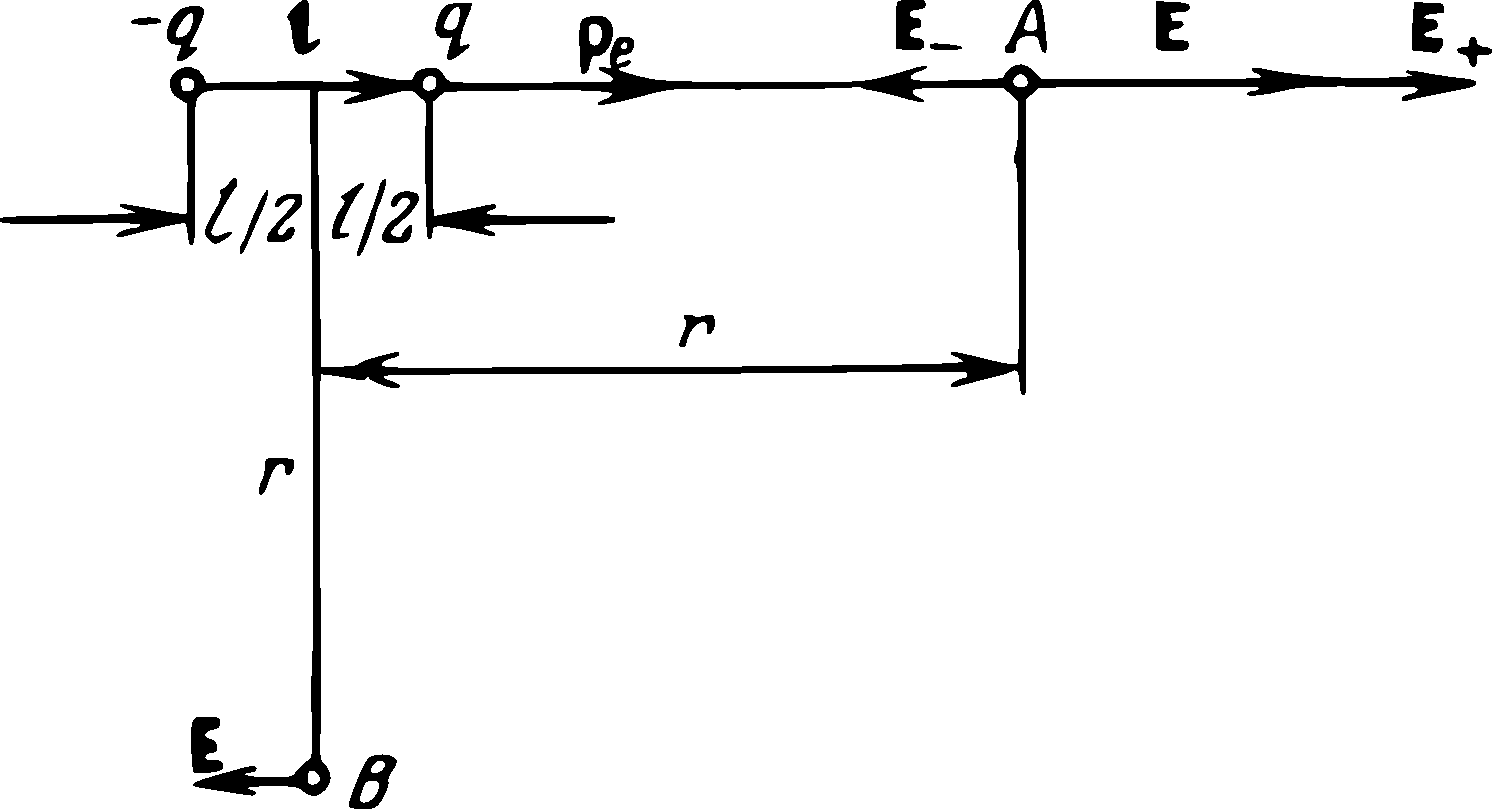
\includegraphics[width=\textwidth]{figs/ch-15/fig-15-01.pdf}
\caption{Electric dipole moment.\zhcap{电偶极矩。}\label{fig-15-01}}
\end{marginfigure}
The strength E of the field of an electric dipole at an arbitrary point is:
\zhpar{电偶极子在任意点的场强 $\vb{E}$ 为：}
\begin{equation*}%
\vb{E} = \vb{E}_{+} + \vb{E}_{-}
\end{equation*}
where $\vb{E}_{+}$ and $\vb{E}_{-}$ are the strengths of the fields set up by the charges $q$ and $-q$ (\figr{fig-15-01}).
At point $A$, located on the dipole axis at the distance $r$ from its middle (\figr{fig-15-01}) $(r \gg l)$, the strength of the field of a dipole equals:
\zhpar{式中 $\vb{E}_{+}$ 与 $\vb{E}_{-}$ 分别为电荷 $q$ 与 $-q$ 所激发的场强（见\figr{fig-15-01}）。在偶极子轴线上、距其中点为 $r$ 的点 $A$ 处（见\figr{fig-15-01}）$(r \gg l)$，偶极子的场强为：}
\begin{align*}%
\vb{E} & = \ofpe \frac{2 \vb{p}_{e}}{\epsilon_{r} r^{3}} & \text{(in SI units)},\\
\vb{E} & =   \frac{2 \vb{p}_{e}}{\epsilon_{r} r^{3}} &\text{(in cgse units)}.
\end{align*}
\begin{marginfigure}
\centering
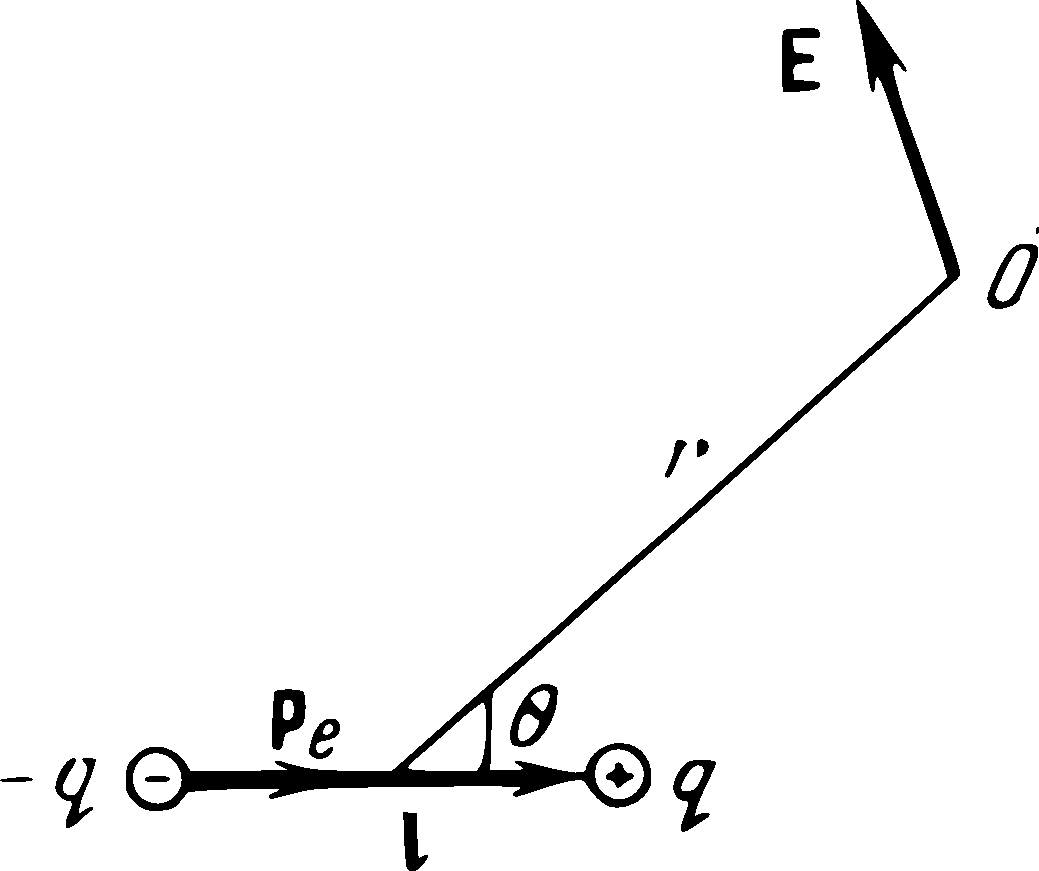
\includegraphics[width=\textwidth]{figs/ch-15/fig-15-02.pdf}
\caption{Electric field strength due to a dipole at an arbitrary point $O$.\zhcap{偶极子在任意点 $O$ 处产生的电场强度。}\label{fig-15-02}}
\end{marginfigure}
At point $B$, located on a perpendicular erected at the middle of the dipole axis and at the distance $r$ from the middle of the axis $(r \gg l)$
\zhpar{在过偶极子轴线中点的垂线上、距该中点为 $r$ 的点 $B$ 处 $(r \gg l)$，场强为}
\begin{align*}%
\vb{E} & = -\, \ofpe \frac{\vb{p}_{e}}{\epsilon_{r} r^{3}} & \text{(in SI units)},\\
\vb{E} & =  - \frac{\vb{p}_{e}}{\epsilon_{r} r^{3}} &\text{(in cgse units)}.
\end{align*}
At the arbitrary point $O$ sufficiently distant from the dipole $(r \gg l)$ (\figr{fig-15-02}), the magnitude of its field strength is:
\zhpar{在距偶极子足够远（$r \gg l$）的任意点 $O$ 处（见\figr{fig-15-02}），场强的大小为：}
\begin{align*}%
\vb{E} & =  \ofpe \frac{{p}_{e}}{\epsilon_{r} r^{3}} \sqrt{3 \cos^{2} \theta + 1} & \text{(in SI units)},\\
\vb{E} & =  - \frac{{p}_{e}}{\epsilon_{r} r^{3}} \sqrt{3 \cos^{2} \theta + 1} & \text{(in cgse units).}
\end{align*}
 
\section{Electric Displacement. Ostrogradsky-Gauss Electric Flux Theorem}
\label{sec-15.3}
\zhtitle{电位移。奥斯特罗格拉茨基-高斯电通量定理}

\subsection{}\label{15.3.1} The electric field strength \ssect{15.1.3} depends upon the properties of the medium. In a homogeneous isotropic medium, the strength $\vb{E}$ is inversely proportional to $\epsilon_{r}$ \ssect{14.2.5}. Another characteristic of an electric field, along with its strength $\vb{E}$, is the vector $\vb{D}$ of \redem{electric displacement}, or \redem{electric induction} (other names are dielectric displacement, dielectric flux density, displacement, electric displacement density and electric flux density). For a field in an electrically isotropic medium, the relation between $\vb{D}$ and $\vb{E}$ is of the form
\zhpar{电场强度 \ssect{15.1.3} 取决于介质的性质。在均匀各向同性介质中，场强 $\vb{E}$ 与 $\epsilon_{r}$ 成反比 \ssect{14.2.5}。除场强 $\vb{E}$ 外，电场的另一特征量是\redem{电位移}（或称\redem{电感应强度}）矢量 $\vb{D}$（其他名称还有：介质电位移、介质电通量密度、位移、电位移密度和电通量密度）。对于电各向同性介质中的电场，$\vb{D}$ 与 $\vb{E}$ 之间的关系为：}
\begin{align*}%
\vb{D} & =  \epsilon_{0}\epsilon_{r} \vb{E} & \text{(in SI units)},\\
\vb{D} & =  \epsilon_{r} \vb{E} & \text{(in cgse units)}.
\end{align*}
The general relation for $\vb{D}$, valid for anisotropic media is given
in \ssect{18.3.4}.
\zhpar{适用于各向异性介质的 $\vb{D}$ 的一般关系式，见\ssect{18.3.4}。}

\hlblue{Example.} For the field of point electric charge $q$ \ssect{14.2.3}
\zhpar{\hlblue{例3。}点电荷 $q$ 的电场 \ssect{14.2.3} 为}
\begin{align*}%
\vb{D} & =  \frac{1}{4 \pi} \, \frac{q}{r^{3}} \, \vb{r} & \text{(in SI units)},\\
\vb{D} & =  \frac{q}{r^{3}} \, \vb{r} & \text{(in cgse units).}
\end{align*}
The projection of $\vb{D}$ on the direction of radius vector $\vb{r}$, from the point charge to the given point in the field, is
\zhpar{由点电荷指向场中所考察点的径矢 $\vb{r}$ 方向上，$\vb{D}$ 的投影为}
\begin{align*}%
\vb{D} & =  \frac{1}{4 \pi} \, \frac{q}{r^{2}} & \text{(in SI units)},\\
\vb{D} & =   \frac{q}{r^{2}} & \text{(in cgse units).}
\end{align*}

\subsection{}\label{15.3.2} An \redem{element} $\dd \Phi_{e}$ of \redem{electric displacement flux} through an element of surface with the area $\dd S$ is the scalar physical quantity defined by the equation
\zhpar{通过面积为 $\dd S$ 的面元的\redem{电位移通量元} $\dd \Phi_{e}$ 是一个标量物理量，由下式定义：}
\begin{equation*}%
\dd \Phi_{e} = \vb{D}\, \vdot \dd \vb{S} = D \, \dd S \cos \alpha = D_{n}\, \dd S = D \, \dd S_{\perp},
\end{equation*}
where $\vb{D}$ is the displacement vector \ssect{15.3.1}, $\vu{n}$ is a unit vector normal to area $\dd S$, $\dd \vb{S} = \dd S \vu{n}$ is the vector of the element of surface $\dd S$, $D_{n} = D \cos \alpha$ is the projection of vector $\vb{D}$ on the direction of vector $\vu{n}$, $\dd S_{\perp} = \dd S \cos \alpha$ is the area of the projection of the element of surface $\dd S$ on a plane perpendicular to vector $\vb{D}$, and $\alpha$ is the angle between vectors $\vb{D}$ and $\vu{n}$ (\figr{fig-15-03})
\zhpar{式中 $\vb{D}$ 为电位移矢量 \ssect{15.3.1}，$\vu{n}$ 为面元 $\dd S$ 的单位法线矢量，$\dd \vb{S} = \dd S \vu{n}$ 为面元的矢量，$D_{n} = D \cos \alpha$ 为 $\vb{D}$ 在 $\vu{n}$ 方向上的投影，$\dd S_{\perp} = \dd S \cos \alpha$ 为面元 $\dd S$ 在与矢量 $\vb{D}$ 垂直的平面上的投影面积，$\alpha$ 为矢量 $\vb{D}$ 与 $\vu{n}$ 之间的夹角（见\figr{fig-15-03}）。}

\begin{marginfigure}[-4cm]
\centering
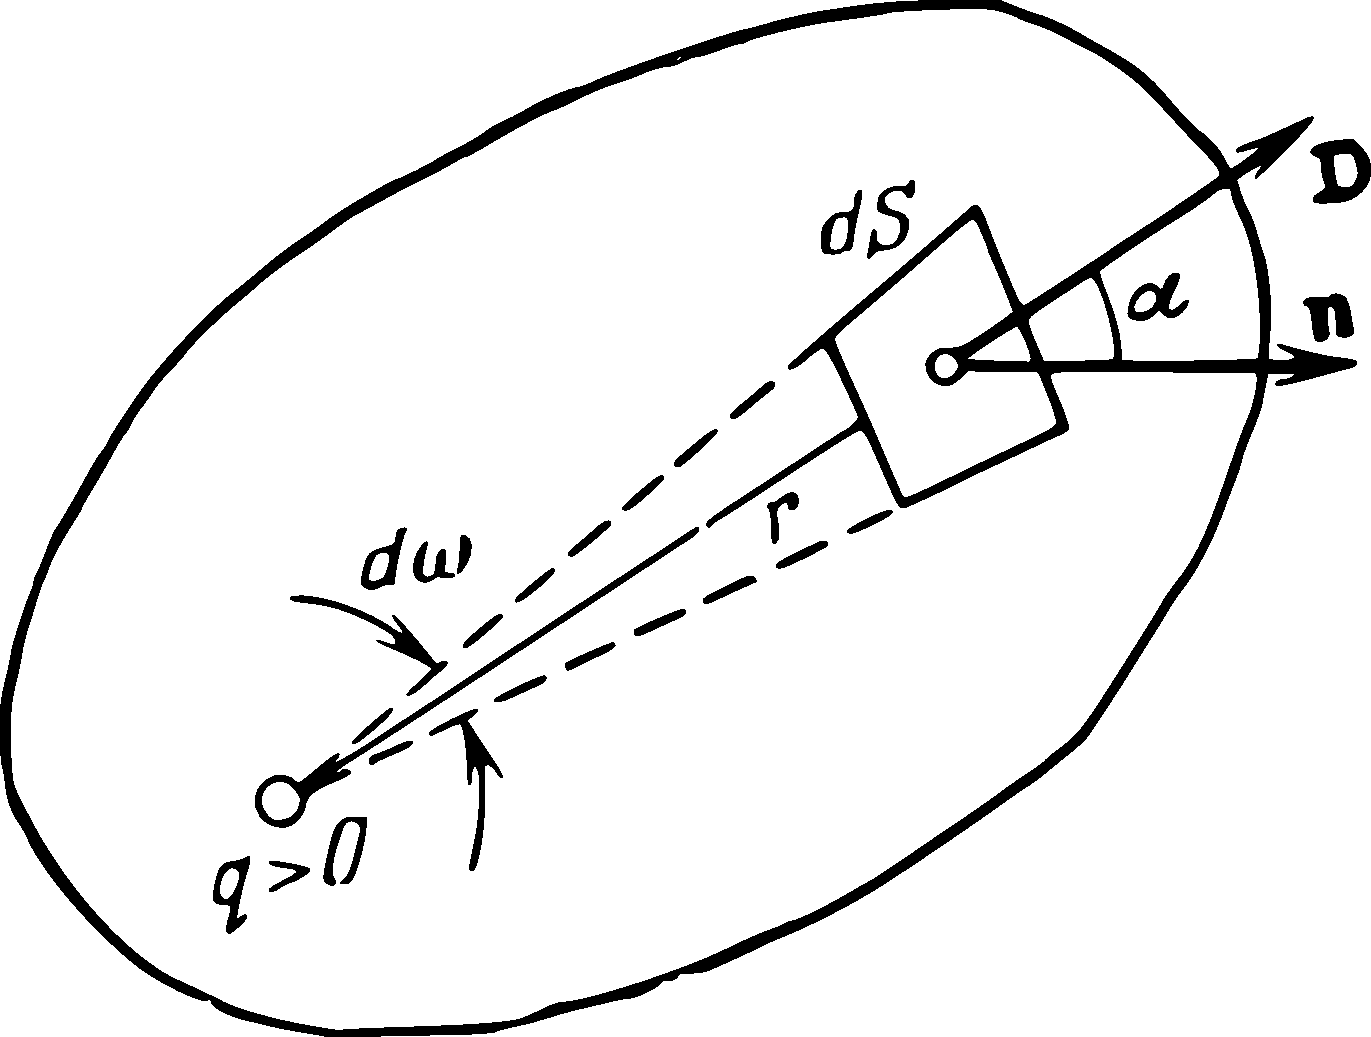
\includegraphics[width=\textwidth]{figs/ch-15/fig-15-03.pdf}
\caption{Electric displacement flux.\zhcap{电位移通量。}\label{fig-15-03}}
\end{marginfigure}

When the electric field is set up by point charge $q$, the element of displacement flux $\dd \Phi_{e}$ through the element of surface $\dd S$ of the closed surface $S$, within which the point charge is located, is
\zhpar{当电场由点电荷 $q$ 激发时，穿过包围该点电荷的闭合曲面 $S$ 上面元 $\dd S$ 的电位移通量元 $\dd \Phi_{e}$ 为}
\begin{equation*}%
\dd \Phi_{e} = \frac{q}{4 \pi} \, \dd \omega,
\end{equation*}
where $\dd \omega$ is the solid angle subtended at point charge $q$ by the element $\dd S$ of surface $S$ (\figr{fig-15-03}).
\zhpar{式中 $\dd \omega$ 为面元 $\dd S$ 对点电荷 $q$ 所张的立体角（见\figr{fig-15-03}）。}

The total \redem{displacement flux} $\Phi_{e}$ through the surface $S$ is the summation or integration of all the elements of flux:
\zhpar{通过曲面 $S$ 的总\redem{电位移通量} $\Phi_{e}$ 等于各通量元的求和（或积分）：}
\begin{align*}%
\Phi_{e} & = \int_{S} \vb{D} \, \dd \vb{S} = \int_{S} {D} \, \dd {S} \cos \alpha \\
& = \int_{S} {D}_{n} \, \dd {S} = \int_{S} {D} \, \dd {S}_{\perp},
\end{align*}
where $\alpha $ is the angle between vectors $\vb{D}$ and $\vu{n}$. Here all the vec­tors and normals to the elements $\dd S$ of surface are directed toward the same side of surface $S$. In the case of a closed surface $S$ (\figr{fig-15-03}), all the vectors n of the normals must be either outward or inward ones.\sidenote{Only outward normals arc used in the following.}
\zhpar{式中 $\alpha$ 为矢量 $\vb{D}$ 与 $\vu{n}$ 之间的夹角。此处，所有矢量以及面元 $\dd S$ 的法线均指向曲面 $S$ 的同一侧。对于闭合曲面 $S$（见\figr{fig-15-03}），所有法线矢量 $\vb{n}$ 都必须指向外侧或都指向内侧。}
\zhpar{注：以下仅采用外法线。}

\subsection{}\label{15.3.3} The \redem{Ostrogradsky-Gauss theorem} states that the displacement flux passing through an arbitrary closed surface is equal to or proportional to the algebraic sum of the electric charges $q_{1},\,q_{2},\, \ldots{}, q_{k}$ enclosed within the surface:
\zhpar{奥斯特罗格拉茨基-高斯定理指出：穿过任意闭合曲面的电位移通量，等于（或正比于）该曲面所包围的电荷 $q_{1},\,q_{2},\, \ldots{}, q_{k}$ 的代数和：}
\begin{align*}%
\oint_{S} \vb{D} \, \dd \vb{S} & = \oint_{S} {D}_{n} \, \dd {S}  = \sum_{i=1}^{k} q_{i} & \text{(in SI units)},\\
\oint_{S} \vb{D} \, \dd \vb{S} & = \oint_{S} {D}_{n} \, \dd {S}  = 4 \pi \sum_{i=1}^{k} q_{i} & \text{(in cgse units).}
\end{align*}
The displacement flux passing through an arbitrary closed sur­face that does not enclose any electric charges equals zero. The differential form of the Ostrogradsky-Gauss theorem is one of Maxwell's equations for an electromagnetic field \ssect{27.4.2}.
\zhpar{穿过任意不包围电荷的闭合曲面的电位移通量等于零。奥斯特罗格拉茨基-高斯定理的微分形式是电磁场麦克斯韦方程组中的一个方程 \ssect{27.4.2}。}

\subsection{}\label{15.3.4} The Ostrogradsky-Gauss theorem for the electrostatic field in vacuum states that vector flux of electrostatic field strength in vacuum passing through an arbitrary closed surface is proportional to the algebraic sum of the electric charges enclosed within the surface:
\zhpar{真空中静电场的奥斯特罗格拉茨基-高斯定理表明：穿过任意闭合曲面的真空中静电场场强的矢量通量，与该曲面所包围的电荷的代数和成正比：}
\begin{align*}%
\oint_{S} \vb{E} \, \dd \vb{S} & = \frac{1}{\epsilon_{0}} \sum_{i=1}^{k} q_{i} & \text{(in SI units),}\\
\oint_{S} \vb{E} \, \dd \vb{S} & = 4 \pi \sum_{i=1}^{k} q_{i}& \text{(in cgse units)}.
\end{align*}
where $\epsilon_{0}$ is the electric constant \ssect{14.2.7}.
\zhpar{式中 $\epsilon_{0}$ 为电常量（真空电容率）\ssect{14.2.7}。}

The Ostrogradsky-Gauss theorem for the field in a dielectric is discussed in \ssect{18.3.3}.
\zhpar{电介质中场的奥斯特罗格拉茨基-高斯定理见\ssect{18.3.3}。}

\subsection{}\label{5.3.5} Together with the principle of superposition of fields \ssect{15.2.2}, the Ostrogradsky-Gauss theorem is applied to calculate electric field vectors $\vb{D}$. This is done by choosing a closed surface in such a way that in the expression for the displacement flux, the quantity $\vb{D}$ can be placed outside the sign of the surface integral. This can be done for fields set up by the simplest symmetrically arranged charges (charged lines, plane, sphere, etc.).
\zhpar{结合场的叠加原理 \ssect{15.2.2}，奥斯特罗格拉茨基-高斯定理可用于计算电位移矢量 $\vb{D}$。为此，应选取恰当的闭合曲面，使电位移通量表达式中的 $\vb{D}$ 可以提到面积分号之外。这种方法适用于由最简单的对称分布电荷（带电直线、平面、球面等）所激发的场。}